
% Thuật toán, pseudocode và flowchart	
\chapter{Thuật toán, mã giả và luồng hoạt động}


\section{Thuật toán mã hoá đối xứng}

Trong lĩnh vực An toàn thông tin, dù đã từng có nhiều thuật toán mã hóa đối xứng được nghiên cứu, phát triển và ứng dụng, nhưng AES (Advanced Encryption Standard) là đang khẳng định vị thế là \textbf{tiêu chuẩn vàng} trong mật mã học hiện đại. Đây là thuật toán mã hóa đối xứng được phát triển và công bố bởi Viện Tiêu chuẩn và Công nghệ quốc gia Hoa Kỳ (NIST) vào ngày 26 tháng 11 năm 2001. \nocite{1250456}


AES khắc phục yếu điểm của DES (Data Encryption Standard) về độ dài khóa. Trong khi DES dễ dàng bị tấn công vét cạn (brute-attack) vì chỉ hỗ trợ độ dài khóa 56bit, AES hỗ trợ linh hoạt với các độ dài khóa như 128, 192 và 256bit, mang lại khả năng bảo mật mạnh mẽ hơn đáng kể. AES xử lý dữ liệu theo khối 128bit tối ưu hơn so với DES chỉ sử dụng khối nhỏ 64bit. Ngoài ra, DES hiện nay đã bị loại bỏ vì thiết kế lỗi thời cũng như dễ dàng bị khai thác các lỗ hổng bảo mật.

AES chính là tiêu chuẩn bảo mật hiện nay được khuyến nghị bởi NIST, nhờ vào các ưu điểm tính ổn định và an toàn hơn so với DES, kiến trúc hiện đại đảm bảo hệ thống kháng cự trước các cuộc tấn công phân tích mật mã (cryptanalytic attacks). \nocite{geeksforgeeks_2025b}

\subsection{Các chế độ mã hóa khối}

Mã hóa khối phân ra các chế độ hoạt động khác nhau, tùy vào cách sử dụng và ứng dụng các Mã hóa khối ấy:

\begin{itemize}
	\item \textbf{Electronic Code Block (ECB}): ECB là một chế độ mã hóa khối đơn giản. Dễ dàng vì chúng mã hóa trực tiếp đầu vào từng khối và đầu ra ở các dạng khối bản mã. Nếu một tin nhắn có kích thước lớn hơn $n$~ bit, chúng sẽ được chia ra thành các khối nhỏ hơn và được xử lý theo tuần tự. \nocite{geeksforgeeks_2025d}
	
	\begin{figure}[H]
		\centering
		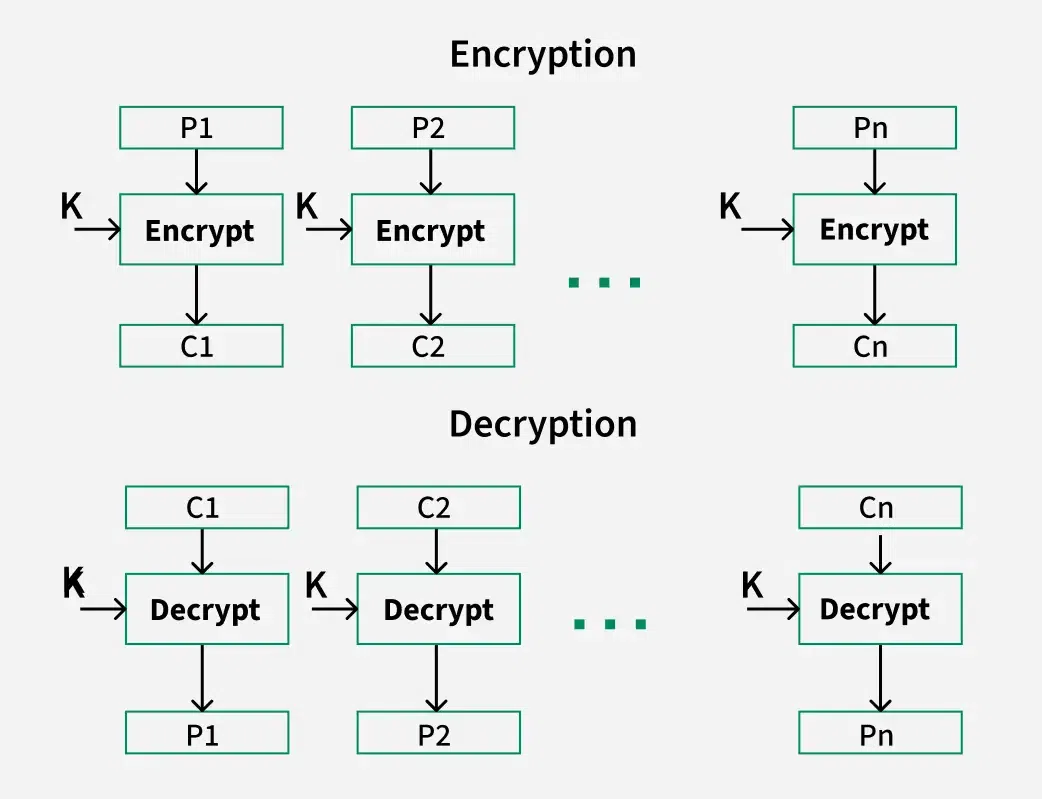
\includegraphics[width=0.8\textwidth]{flowcharts/ecb.png} 
		\caption{Chế độ hoạt động mã khối ECB} 
		\label{fig:ecb_block}
	\end{figure}
	
	\item \textbf{Cipher Block Chaining (CBC)}:
	 CBC là một cải tiến dựa trên ECB, bởi vì ECB dễ bị phá vỡ. Trong CBC, khối mã hóa trước đó là đầu vào cho thuật toán mã hóa tiếp theo sau khi thực hiện XOR với khối bản rõ gốc. Nói tóm lại, bản mã khối được tạo ra bằng cách mã hóa kết quả XOR giữa bản mã khối trước đó và khối bản rõ hiện tại. 
	
		\begin{figure}[H]
		\centering
		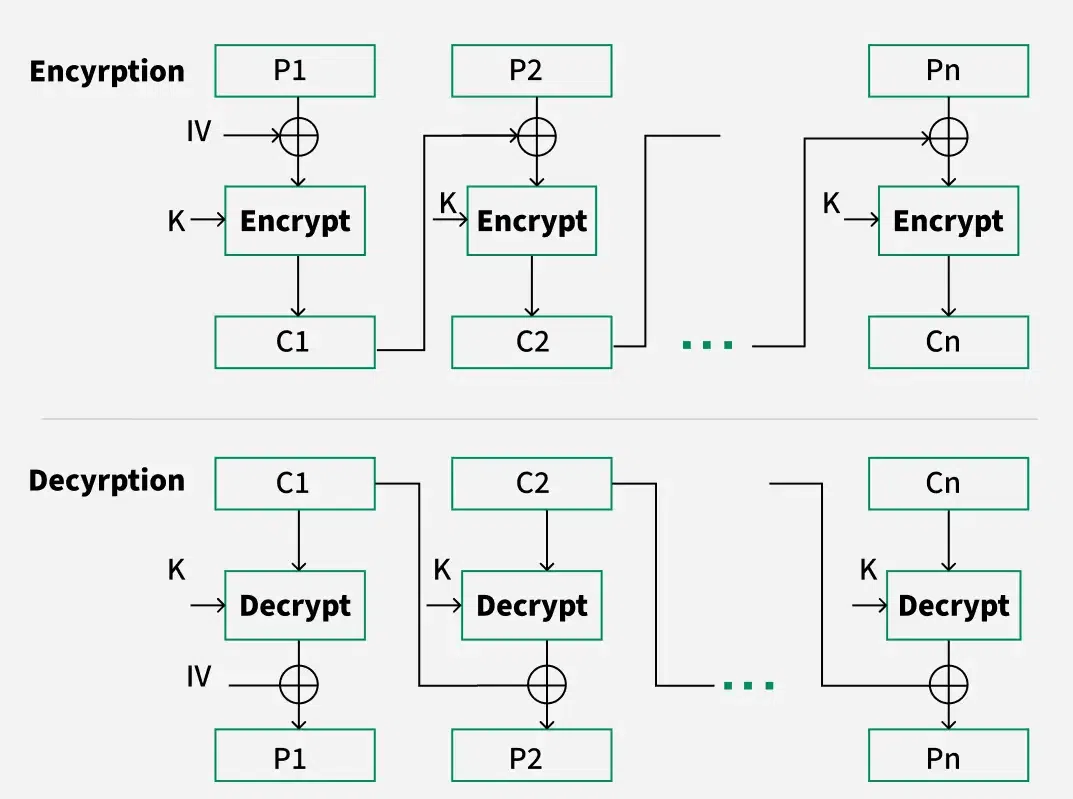
\includegraphics[width=0.8\textwidth]{flowcharts/cbc.png} 
		\caption{Chế độ hoạt động mã khối CBC} 
		\label{fig:cbc_block}
	\end{figure}
	
	\item \textbf{Cipher Feedback Mode (CFB)}:
	Trong CFB, mật mã được cung cấp dưới dạng phản hồi cho khối mã hóa tiếp theo với một số thông số kĩ thuật mới. Đầu tiên, một vector khởi tạo $IV$ được sử dụng cho lần mã hóa đầu tiên và đầu ra có kích thước $b$ bit được chia thành hai phần: $s$ bit bên trái và $s-b$ bit bên phải. Phía bên trái của đầu ra có kích thước $s$ bit thực hiện $XOR$ với bản rõ khối hiện tại. Kết quả của phép $XOR$ sẽ là đầu vào của thanh ghi dịch (shift register) có $b-s$~ bit cũ được dịch phía bên trái, và nạp $s$~bits của phép XOR trước đó vào phía bên phải và quy trình hoạt động cứ thế lặp lại cho các khối tiếp theo.     
	
	\begin{figure}[H]
		\centering
		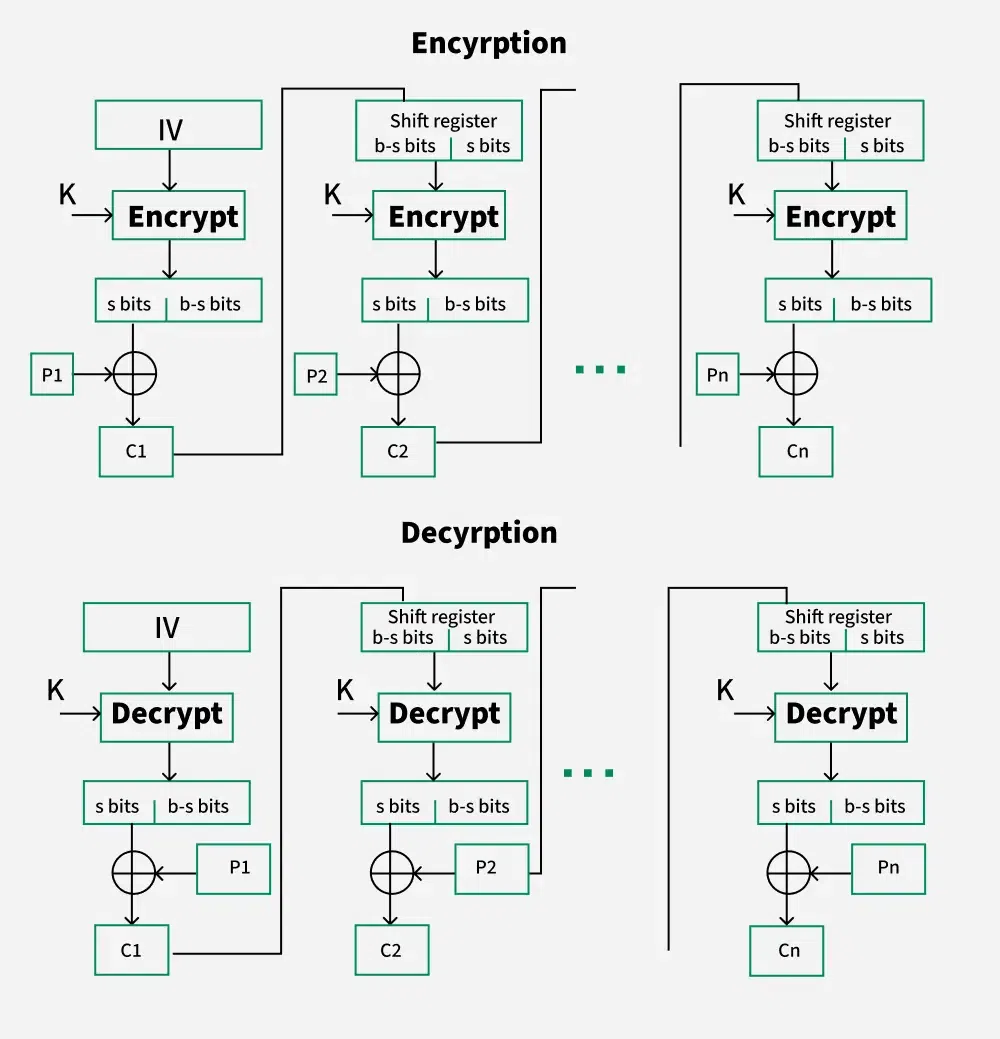
\includegraphics[width=0.8\textwidth]{flowcharts/cfb.png} 
		\caption{Chế độ hoạt động mã khối CFB} 
		\label{fig:cfb_block}
	\end{figure}
	
		\item \textbf{Output Feedback Mode (OFB)}:
	OFB cũng có quy trình hoạt động gần tuân thủ theo chế độ CFB ngoại trừ việc nó sẽ gửi đầu ra bản mã làm phản hồi thay vì gửi đầu ra của phép XOR như CFB.  
	
	\begin{figure}[H]
		\centering
		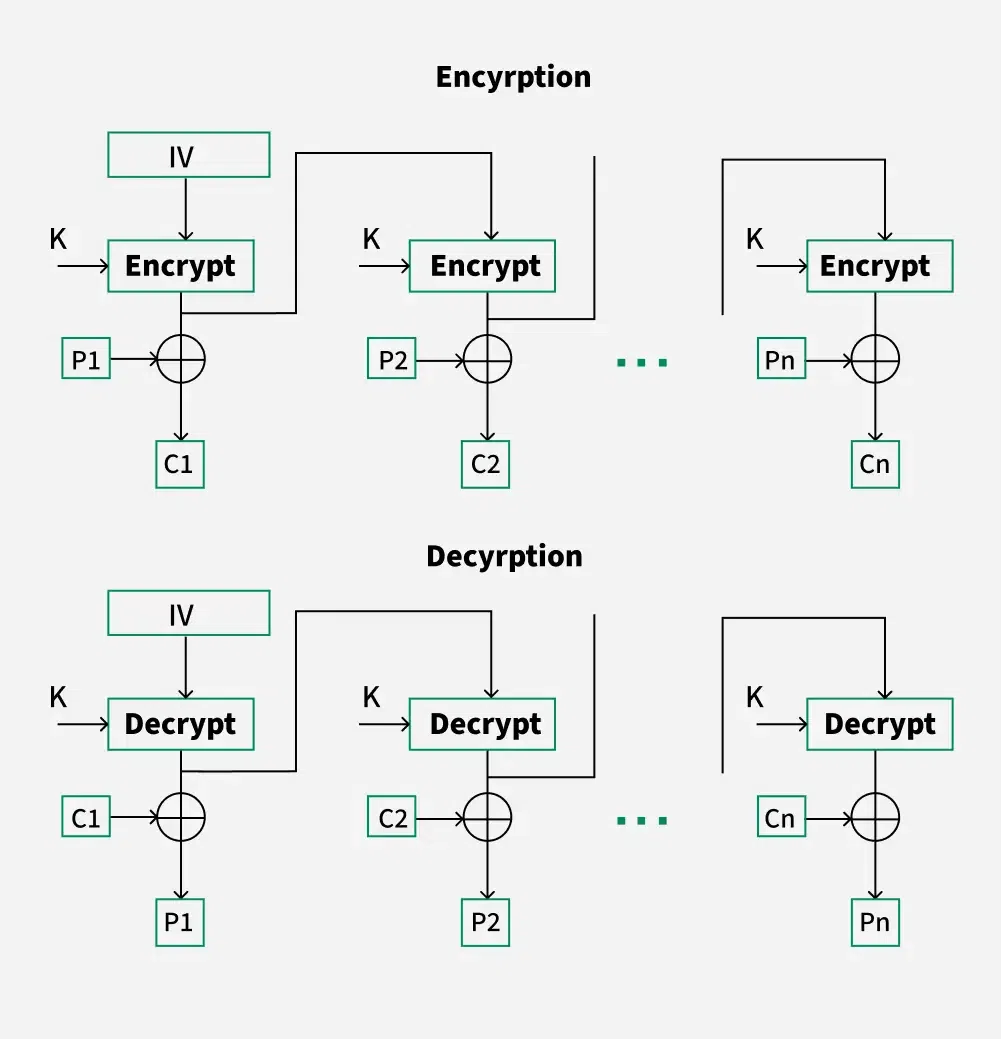
\includegraphics[width=0.8\textwidth]{flowcharts/ofb.png} 
		\caption{Chế độ hoạt động mã khối OFB}
		\label{fig:ofb_block}
	\end{figure}
	
		
	\item \textbf{Counter Feedback Mode (CTR)}:
	CTR triển khai mật mã khối dựa trên một bộ đếm đơn giản. Mỗi lần một giá trị đếm khởi tạo ngược được mã hóa và là đầu vào của phép $XOR$ với bản rõ và đầu ra của phép này là một khối mã hóa. CTR độc lập trong hoạt động sử dụng phản hồi nên chúng có được thực hiện song song.
	
	\begin{figure}[H]
		\centering
		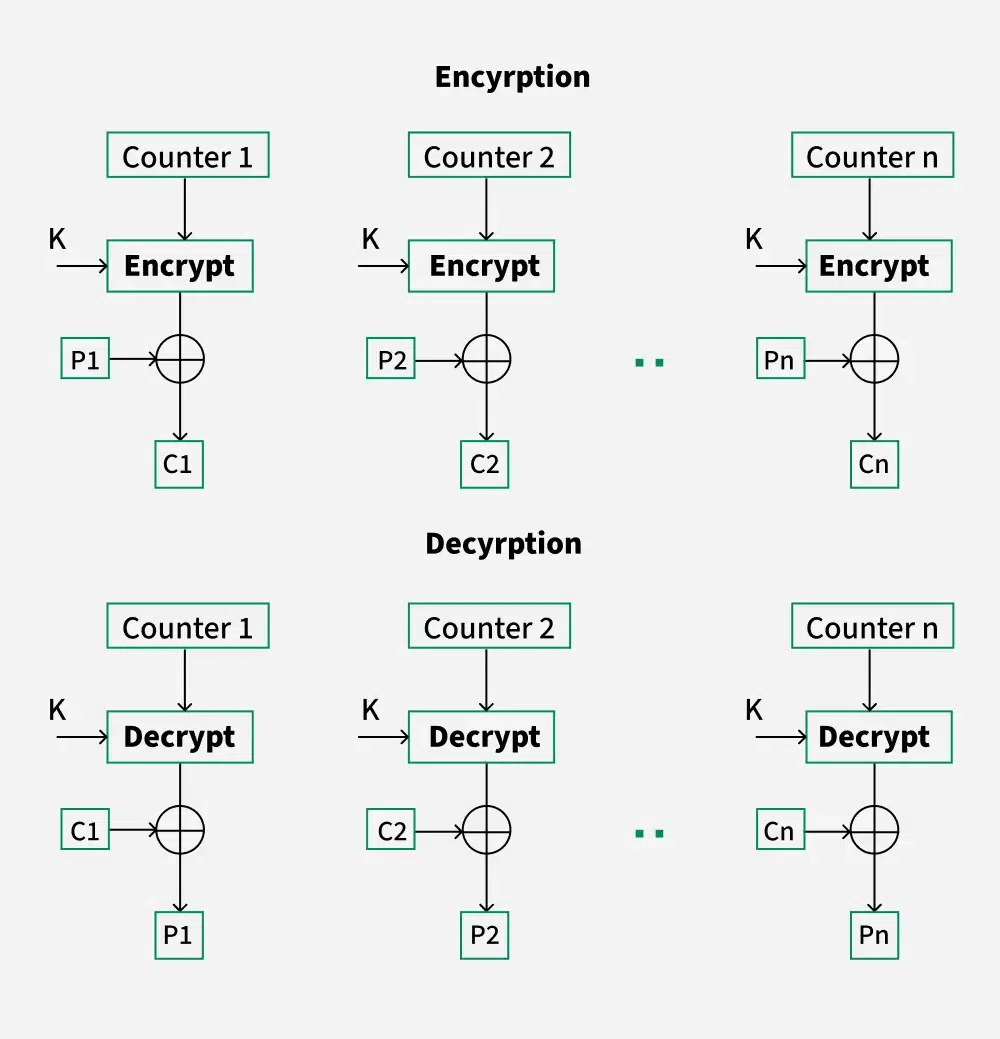
\includegraphics[width=0.8\textwidth]{flowcharts/ctr.png} 
		\caption{Chế độ hoạt động mã khối CTR}
		\label{fig:ctr_block}
	\end{figure}
	
\end{itemize} 

\subsection{Nguyên lý hoạt động}

Thuật toán AES được thiết kế dựa trên cấu trúc mạng Thay thế - Hoán vị (Substitution - Permutation Network). Cấu trúc mạng này biến đổi, xử lý giữa bản rõ và khóa theo khối qua các vòng lặp xen kẽ giữa hai lớp chính: Lớp thay thế (\textbf{S-layers}) và Lớp Hoán vị (\textbf{P-layers}) nhằm sinh ra văn bản đã được mã hóa. \nocite{KONG201515}

\subsubsection{Kích thước đầu vào}

Theo đề án nguyên bản của Rijmen và Daemen \nocite{Daemen:2002:DRA}, \textbf{Rijndael} là một mật mã khối lặp đi lặp lại với kích thước khối và kích thước khóa khác nhau. Rijndael hỗ trợ kích thước khối, kích thước khóa độc lập nhau với các giá trị 128, 192 hoặc 256~bit. 

Tuy nhiên, khi thuật toán AES được chuẩn hóa theo Viện Tiêu chuẩn và Công nghệ quốc gia (FIPS197), đầu vào của thuật toán AES (tức là kích thước bản khối) là 128~bit, trong khi kích thước khóa có thể tương thích với các giá trị 128, 192 hoặc 256~bit. \nocite{1250456}

\subsubsection{Ma trận trạng thái}

Các phép biến đổi khác nhau với một kết quả trung gian, còn được gọi là \textbf{Trạng thái} (State).

\textbf{Ma trận trạng thái} là một mảng các bytes được biểu diễn dưới dạng hình chữ nhật. Mảng này có bốn hàng, số cột tương ứng được kí hiệu là $N_b$, và chúng tương ứng với kích thước của bản khối chia hết cho 32. (128, 192 và 256~bit tương ứng với số cột là 4, 6, 8). \nocite{Daemen:2002:DRA}

\subsubsection{Số chu kỳ}
Số chu kỳ của Rijndael phụ thuộc vào giá trị của $N_b$ và $N_k$:
\begin{table}[h]
	\centering
	\caption{Số chu kỳ thực hiện thuật toán dựa theo $N_r$ và $N_b$}
	\begin{tabular}{|c|c|c|c|}
		\hline
		$N_r$ & $N_b = 4$ & $N_b = 6$ & $N_b = 8$ \\ \hline
		$N_k = 4$ & 10 & 12 & 14 \\ \hline
		$N_k = 6$ & 12 & 12 & 14 \\ \hline
		$N_k = 8$ & 14 & 14 & 14 \\ \hline
	\end{tabular}
\end{table}

\subsubsection{Quy trình mã hóa/giải mã}

Giải thuật AES thực hiện mã hóa khối dữ liệu thông qua các bước xử lý chính như sau:

\begin{enumerate}[label= \textbf{Bước \arabic*:}]
	\item Mở rộng khóa nhằm thực hiện sinh các khóa vòng (Round key), dùng trong các vòng lặp từ khóa chính sử dụng thủ tục sinh khóa \textbf{Rijndael}.
	\item Vòng khởi tạo sẽ thực hiện hàm AddRoundKey, trong đó mỗi byte trong State được kết hợp với khóa vòng sử dụng phép XOR.
	\item Với mỗi lặp chính, mỗi vòng sẽ bao gồm 4 hàm chính xử lý dữ liệu như sau:
	\begin{itemize}
		\item Tiến hành thay thế phi tuyến tính sử dụng hàm \textbf{SubBytes}, trong đó mỗi bytes trong state được thay thế bằng bytes khác sử dụng bảng tham chiếu S-box.

		\item Mỗi dòng trong state được dịch một số bước theo chu kỳ, sử dụng hàm \textbf{ShiftRows}.
		\item \textbf{MixColumns} làm trộn các cột trong state, kết hợp 4 bytes trong mỗi cột. 
		\item \textbf{AddRoundKeys} là hàm kết hợp state với khóa vòng, sử dụng phép XOR.
	\end{itemize}
	\item Vòng lặp cuối cùng cũng tương tự các vòng chính khác, nhưng không thực hiện bước \textbf{MixColumns}.
\end{enumerate}

Với quá trình giải mã, giải thuật AES khôi phục bản rõ bằng cách sử dụng hàm ngược của các phép biến đổi đã được sử dụng ở quy trình mã hóa, và thực hiện các hàm ấy theo trình tự ngược so với mã hóa. Đồng thời, các khóa vòng cũng được sử dụng theo hướng lui về dần từ khóa vòng cuối cùng về khóa gốc ban đầu.

\subsection{Mã hoá / Giải mã}

\subsubsection{Quy trình sinh khóa vòng}

Các khóa vòng có nguồn gốc từ Khóa mã hóa và chúng được tạo thông qua quy trình lập lịch khóa. Quy trình này bao gồm hai thành phần chính: sinh khóa chính và lựa chọn khóa vòng. Các nguyên tắc cơ bản của thuật toán như sau:
\begin{itemize}
	\item Tổng số bit của toàn bộ RoundKey phải bằng độ dài của bản khối nhân với số vòng cộng thêm 1 (ví dụ một bản khối có kích thước 128~bit và 10 vòng, thì tổng số bit của các RoundKey phải là 1408~bit).
	\item Bản khóa mã hóa được mở rộng thành Khóa mở rộng (Expended Key).
	\item Các khóa vòng được lấy ra từ Khóa mở rộng như sau: Khóa vòng đầu tiên phải chứa $N_b$ từ đầu tiên, khóa vòng thứ hai chứa $N_b$ và tương tự cho các khóa vòng tiếp theo.
\end{itemize}

\paragraph{a. Thủ tục sinh khóa}\quad

Khóa mở rộng (Expended Key) là một mảng tuyến tính gồm các từ 4 byte và được ký hiệu: $W[N_b * (N_r+1)]$. $N_k$ từ đầu tiên bao gồm bản mã khóa gốc. Các từ còn lại được định nghĩa một cách đệ quy. 

Thủ tục sinh khóa phụ thuộc vào chiều dài của khóa $N_k$. Chính vì vậy, có hai phiên bản thủ tục sinh khóa: một dành cho $N_k \leq 6$ và một dành cho $N_k > 6$. Với phiên bản $N_k \leq 6$, ta có mã giả:

\begin{center}
	\begin{BVerbatim}
KeyExpansion(byte Key[4*Nk] word W[Nb*(Nr+1)])
{
	for(i = 0; i < Nk; i++)
		W[i] = (Key[4*i],Key[4*i+1],Key[4*i+2],Key[4*i+3]);
	
	for(i = Nk; i < Nb * (Nr + 1); i++)
	{
		temp = W[i - 1];
		if (i % Nk == 0)	
		temp = SubByte(RotByte(temp)) ^ Rcon[i / Nk];
		W[i] = W[i - Nk] ^ temp;
	}
}
	\end{BVerbatim}
\end{center}

Trong mã giả trên, $SubByte(W)$ là một hàm trả về một từ 4 byte với mỗi byte từ đầu vào, được thay thế tương ứng với bảng thay thế (S-box). 

Hàm $RotByte(W)$ thực hiện hoán vị các bytes của từ theo chu kỳ. Giả sử đầu vào là $(a,b,c,d)$ thì đầu ra của hàm sẽ là $(b,c,d,a)$.

Có thể thấy rằng $N_k$ từ đầu tiên chính là bản mã khóa (Cipher Key). Các từ tiếp theo $W[i]$ chính là kết quả của phép XOR giữa từ ở vị trí trước đó $W[i-1]$ và từ cách $W[i]$ một khoảng $N_k$ ($W[i-N_k]$).

Đối với những từ ở vị trí là bội số của $N_k$, việc chuyển đổi này được áp dụng với $W[i-1]$, sau đó $W[i-1]$ này sẽ thực hiện XOR với một hằng số vòng tương ứng. Quá trình chuyển đổi bao gồm dịch chuyển các byte trong 1 từ ($RotByte$), sau đó là thay thế các giá trị byte này theo bảng thay đổi (S-box) ($SubByte$).

Các hằng số vòng độc lập với $N_k$ được định nghĩa như sau:
\begin{center}
	$Rcon[i] = (RC[i], \{00\}, \{00\}, \{00\})$
\end{center}
với  $RC[i]$ là một phần tử trong trường hữu hạn $GF(2^8)$ với giá trị $x(i-1)$:
\begin{align*}
	RC[1] &= 1~ \text{(Tức là \{01\})} \\
	RC[i] &= x~ \text{(Tức là \{02\})}~ .(RC[i-1]) = x(i-1)
\end{align*}

Với $N_k > 6$, ta có mã giả:
\begin{center}
	\begin{BVerbatim}
	KeyExpansion(byte Key[4*Nk] word W[Nb*(Nr+1)])
	{	
		for(i = 0; i < Nk; i++)
			W[i] = (key[4*i],key[4*i+1],key[4*i+2],key[4*i+3]);
		
		for(i = Nk; i < Nb * (Nr + 1); i++)
		{
			temp = W[i - 1];	 
		 	if (i % Nk == 0)		
		 		temp = SubByte(RotByte(temp)) ^ Rcon[i / Nk];	
		 	else if (i % Nk == 4) 			
				temp = SubByte(temp);
				
		 	W[i] = W[i - Nk] ^ temp;
		}
	}
	\end{BVerbatim}
\end{center}
Điểm khác biệt so với các phiên bản có $N_k \leq 6$ là thêm một bước xử lý tại các vị trí $(i - 4)$ là bội số của $N_k$, hàm \textbf{SubWord} sẽ được áp dụng cho $W[i-1]$ trước khi thực hiện phép XOR.
 
\paragraph{b. Lựa chọn khóa vòng}\quad

Khóa vòng được chọn ra từ bộ đệm khóa vòng từ $W[i*N_b]$ đến $W[i*(N_b+1)]$. 

\subsubsection{Quy trình mã hóa}

Các vòng chuyển đổi của thuật toán AES qua bốn phép chuyển đổi khác nhau, được trình bày thông qua đoạn mã giả:
\begin{center}
	\begin{BVerbatim}
	Round(State,RoundKey)
	{
		ByteSub(State);
		ShiftRow(State);
		MixColumn(State);
		AddRoundKey(State,RoundKey);
	}
	\end{BVerbatim}

\end{center}

Ở vòng cuối cùng của thuật toán, sẽ không thực hiện phép biến đổi \texttt{MixColumn}:
\begin{center}
	\begin{BVerbatim}
	FinalRound(State,RoundKey)
	{
		ByteSub(State) ;
		ShiftRow(State) ;
		AddRoundKey(State,RoundKey);
	}
	\end{BVerbatim}
\end{center}

\paragraph{a. \texttt{ByteSub}}\quad

Phép biến đổi \texttt{ByteSub} là phép biến đổi thay thế phi tuyến tính được thực hiện cho từng byte của ma trận trạng thái một cách độc lập. Bảng thay thế (S-box) có thể đảo ngược và được xây dựng như một thành phần giữa hai quá trình biến đổi:
		\begin{itemize}
	\item Một phép nhân nghịch đảo trong trường hữu hạn $GF(2^8)$ được tính theo modulo một đa thức $m(x) = x^8 + x^4 + x^3 + x + 1$. $\{00\}$ được phản ánh trong chính nó.
	\item Sau đó, một phép biến đổi \textbf{Affine} được áp dụng và có định nghĩa như sau:
	
	\begin{align}
		\begin{bmatrix} 
			y_0\\y_1\\ y_2\\y_3\\y_4\\y_5\\y_6\\y_7
		\end{bmatrix} &= 
		\begin{bmatrix}
			1 & 0 & 0 & 0 & 1 & 1 & 1 & 1\\
			1 & 1 & 0 & 0 & 0 & 1 & 1 & 1\\
			1 & 1 & 1 & 0 & 0 & 0 & 1 & 1\\
			1 & 1 & 1 & 1 & 0 & 0 & 0 & 1\\
			1 & 1 & 1 & 1 & 1 & 0 & 0 & 0\\
			0 & 1 & 1 & 1 & 1 & 1 & 0 & 0\\
			0 & 0 & 1 & 1 & 1 & 1 & 1 & 0\\
			0 & 0 & 0 & 1 & 1 & 1 & 1 & 1\\
		\end{bmatrix}
		\begin{bmatrix} 
			x_0\\x_1\\x_2\\x_3\\x_4\\x_5\\x_6\\x_7
		\end{bmatrix}
		+
		\begin{bmatrix}
			1\\1\\0\\0\\0\\1\\1\\0
		\end{bmatrix}
	\end{align}
	
\end{itemize}

\paragraph{b. \texttt{ShiftRow}}\quad

Các hàng trong trạng thái được dịch chuyển theo chu kỳ tùy thuộc vào hệ số quay $C$ khác nhau. Hàng đầu tiên sẽ không dịch chuyển, hàng thứ hai sẽ dịch chuyển $C1$ byte, hàng thứ 3 dịch chuyển $C2$ byte và hàng cuối cùng dịch chuyển $C3$ byte.

Hệ số quay $C1, C2, C3$ phụ thuộc vào độ dài khối $N_b$. 
\begin{table}[h]
	\centering
	\caption{Hệ số quay phụ thuộc vào các giá trị $N_b$ khác nhau}
	\begin{tabular}{|c|c|c|c|}
		\hline
		$N_b$ & $C1$ & $C2$ & $C3$ \\ \hline
		$4$ & 1 & 2 & 3 \\ \hline
		$6$ & 1 & 2 & 3 \\ \hline
		$8$ & 1 & 4 & 4 \\ \hline
	\end{tabular}
\end{table}

\paragraph{c. \texttt{MixColumn}}\quad

\textbf{MixColumns} làm trộn các cột trong states, kết hợp 4 bytes trong mỗi cột. 
Các cột trạng thái được coi là đa thức trong $GF(2^8)$ và nhân theo modulo $x^4+1$ với một đa thức cố định: $c(x)='03'x^3+'01'x^2+'01'x+02$ nghịch đảo.

Biến đổi này có thể được biểu diễn như một phép nhân trong ma trân, với mỗi bytes là một phần tử trong trường $GF(2^8)$. Cho $b(x) = c(x) \times a(x)$:
\begin{center}
	$\begin{bmatrix} b_0 \\ b_1 \\b_2 \\ b_3\end{bmatrix} =
	\begin{bmatrix}
		02 & 03 & 01 & 01 \\
		01 & 02 & 03 & 01 \\
		01 & 01 & 02 & 03\\
		03 & 01 & 01 & 02 \\
	\end{bmatrix}
	\begin{bmatrix} a_0 \\ a_1 \\ a_2 \\ a_3 \\ \end{bmatrix}$
\end{center}

\paragraph{d. \texttt{AddRoundKey}}\quad

Phép biến đổi này đơn giản là kết hợp state với khóa vòng, sử dụng phép XOR. Chiều dài của khóa vòng bằng chiều dài của khối $N_b$. Phép biến đổi AddRoundKey còn có nghịch đảo là chính nó.

\subsubsection{Quy trình giải mã}

Các phép biến đổi trong quá trình mã hóa của giải thuật AES có thể nghịch đảo được, và thực hiện chúng theo một trình tự đảo ngược so với quy trình mã hóa, ta thu được quá trình giải mã, khôi phục bản rõ từ đầu vào là bản mã hóa và khóa. Quy trình giải mã được trình bày thông qua đoạn mã giả:

\begin{BVerbatim}
	InvCipher(State, CipherKey)
	{
		InvKeyExpension(CipherKey, InvExpendedKey);
		AddRoundKey(State, InvExpendedKey + Nb*Nr);
		for (i = Nr-1; i>0; i--) 
		{
			InvByteSub(State);
			InvShiftRow(State);
			InvMixColumn(State);
			AddRoundKey(State,InvRoundKey);
		}
		InvByteSub(State);
		InvShiftRow(State);
		AddRoundKey(State,RoundKey0); // RoundKey0 tức là khóa gốc
	}
\end{BVerbatim}

Trong đó, quá trình sinh khóa nghịch đảo (\texttt{InvKeyExpension}) được định nghĩa và mã giả như sau:
\begin{enumerate}
	\item Áp dụng giải thuật Sinh khóa (Key Expension).
	\item Áp dụng phép biến đổi MixColumn nghịch đảo (InvMixColumn) cho mọi khóa vòng ngoại trừ khóa khởi tạo và khóa gốc.
\end{enumerate}
\begin{center}
\begin{BVerbatim}
	InvKeyExpansion(CipherKey,InvExpandedKey)
	{
		KeyExpansion(CipherKey,InvExpandedKey);
		for( i=1 ; i < Nr ; i++ )
		InvMixColumn(InvExpandedKey + Nb*i) ;
	}
\end{BVerbatim}
\end{center}


\paragraph{a. \texttt{InvByteSub}}\quad

Đảo ngược phép ByteSub là thay thế byte trong ma trận trạng thái với giá trị tương ứng trong Bảng nghịch đảo ($Inv~S-box$).

Bảng nghịch đảo này thu được bằng cách đảo ngược ánh xạ affine và sau đó thực hiện đảo nghịch phép nhân trong trường hữu hạn $GF(2^8)$.

\paragraph{b. \texttt{InvShiftRow}}\quad

Đảo ngược của ShiftRow là phép dịch chuyển các byte theo chu kỳ. Dòng đầu tiên không dịch chuyển, ba dòng cuối cùng lần lượt được dịch chuyển theo $N_b-C1, N_b-C2$ và $N_b-C3$. Chính vì thế, với byte tại vị trí $j$ ở dòng $i$ sẽ được dịch chuyển đến vị trí tương ứng là $(j + N_b-C_i) \mod N_b$.

\paragraph{c. \texttt{InvMixColumn}}\quad

Đảo ngược của InvMixColumn cũng tương tự như MixColumn. Mỗi cột trong Ma trận trạng thái là một đa thức trong trường hữu hạn $GF(2^8)$ và theo modulo đa thức $x^4+1$, với một đa thức cố định $a^{-1}(x)$:
\begin{center}
	$a^{-1}(x) = \{0b\}x^3 + \{0d\}x^2 + \{09\}x + \{0e\}$
\end{center}

\subsection{Flowchart}

Giải thuật AES với hai quy trình giải mã, mã hóa sẽ được trình bày một cách trực quan thông qua biểu đồ Flowchart \nocite{vlsi2018}:

\begin{figure}[H]
	\centering
	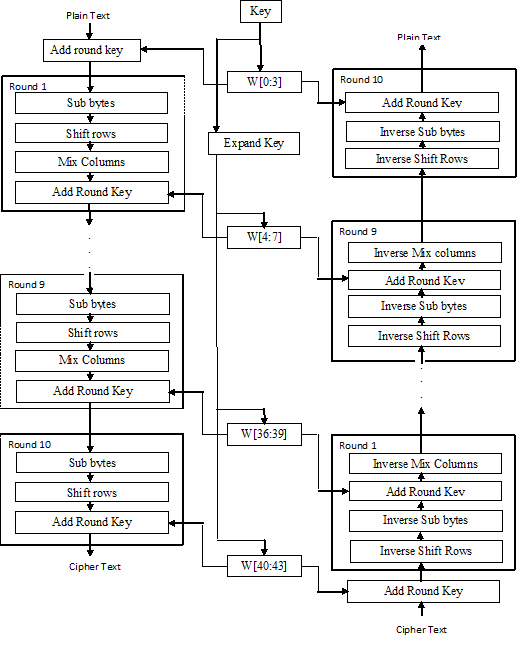
\includegraphics[width=0.8\textwidth]{flowcharts/aes_encrypt_decrypt.png} 
	\caption{Lưu đồ thuật toán AES với bản khối 128~bit và bản khóa 128~bit} 
	\label{fig:flowchart-aes}
\end{figure}

\section{Thuật toán mã hoá bất đối xứng}

Trong các loại thuật toán mã hóa bất đối xứng, nếu như thuật toán \textbf{RSA} nổi tiếng với khả năng bảo mật dựa vào các số nguyên tố lớn thì thuật toán \textbf{ECC} dựa trên cơ sở toán học của \textbf{Đường cong Elliptic}, vẫn đạt được khả năng bảo mật tương đương nhưng chỉ cần khóa nhỏ hơn nhiều.

Thuật toán ECC (Elliptic Curve Cryptography) được phát triển bởi Neal Koblitz và Victor S. Miller vào năm 1985. Hệ mật mã trên đường cong Elliptic có thể thực hiện được các chức năng chính của thuật toán mã hóa đối xứng như: trao đổi khóa, mã hóa và thực hiện chữ ký số. \nocite{geeksforgeeks_2025c}



\subsection{Nguyên lý hoạt động}

\subsubsection{Đường cong Elliptic}

Đường cong Elliptic là đường cong đại số phẳng, là tập hợp tất cả các điểm $\{x,y\}$ trong phương trình tổng quát như sau:
\begin{center}
	$Ax^3 + Bx^2y+ Cxy^2+ Dy^3+Ex^2+Fxy+Gy^2+Hx+Iy+J=0 $
\end{center}

Tuy nhiên, trong mật mã học, các đường cong Elliptic đã được đơn giản hóa (dạng Weierstras), với định nghĩa:
\begin{center}
	$y^2 = x^3 + ax + b$

\end{center} \nocite{inproceedings_85}

\textbf{Ví dụ}: Thuật toán đường cong Elliptic \textbf{secp256k1} ứng dụng trong Bitcoin sử dụng phương trình: $y^2 = x^3 + 7$

\begin{figure}[H]
	\centering
	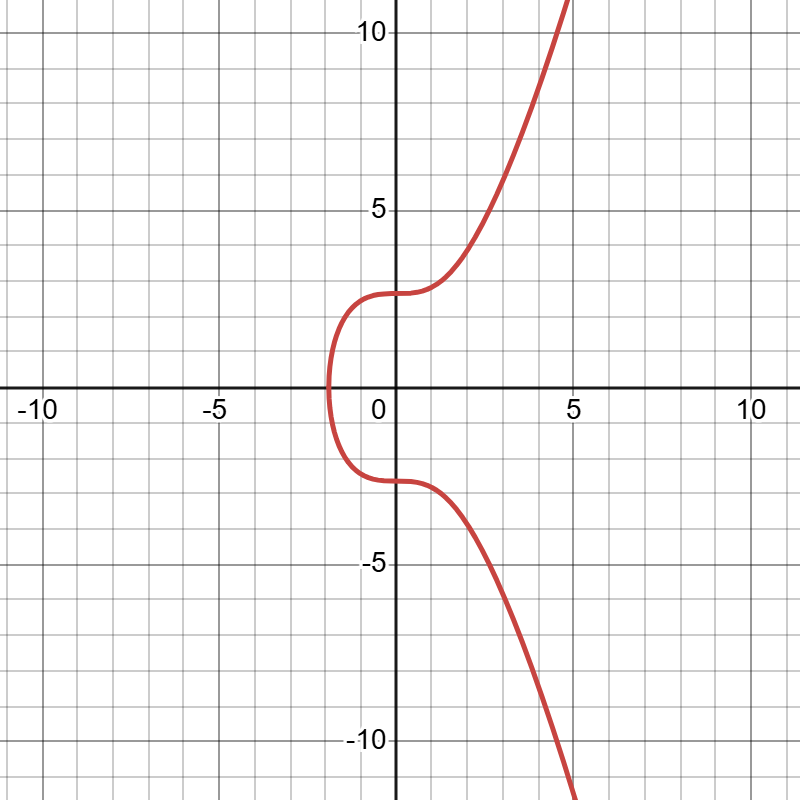
\includegraphics[width=0.8\textwidth]{ecp256k1.png} 
	\caption{Đồ thị trực quan hóa phương trình $y^2 = x^3 + 7$} 
	\label{fig:secp256k1}
\end{figure}

Hệ mật mã trên đường cong Elliptic sử dụng các đường cong trên trường hữu hạn $G_p$ (p là số nguyên tố và p>3) hoặc $G_{2^m}$ (kích thước trường $p = 2^m$). 

Chính vì vậy, khi thực hiện các phép tính đại số như cộng, nhân trong trường hữu hạn, chúng sẽ dẫn đến một điểm khác trong trường. Do đó, phương trình đường cong Elliptic có dạng modulo như sau:
\begin{center}
	$y^2 \equiv x^3 + ax + b (\mod p)$ 
\end{center} 

\subsubsection{Phép tính đường cong Elliptic trên trường hữu hạn}

Để kiểm tra một điểm $\{x,y\}$ có thuộc đường cong Elliptic trên trường hữu hạn nào đó không, ta chỉ cần thế chúng vào một đường cong Elliptic và kiểm tra phương trình đồng dư đó có thỏa mãn hay không.

\textbf{Ví dụ}: Điểm $(5,8)$ thuộc đường cong Elliptic: $y^2\equiv x^3+7 (\mod 17))$ vì $(5^3+7-8^2)\equiv 0 (\mod 17)$





\subsubsection{Nhân điểm trên đường cong ECC với một số nguyên}

Hai điểm trên đường cong EC có thể được thêm vào kết quả là một điểm khác cũng nằm trên đường cong EC. Phép tính này được gọi là phép cộng điểm EC.

Cho một điểm $G$ nào đó trên đường cong trên trường hữu hạn, nếu ta nhân điểm này với một số nguyên $k$ thì ta sẽ thu lại được một điểm EC khác là $P$ cũng nằm trên đường cong trên trường hữu hạn này. 

Phép nhân này có thể được biểu diễn như sau: $P=kG$

\subsection{Mã hoá / Giải mã}

\subsubsection{Khóa ECC}

Bất kỳ một số nguyên nào trong phạm vi kích thước trường của đường cong ECC, cũng đều có thể được sử dụng làm khóa riêng ECC hợp lệ (thông thường là số nguyên 256~bit).

Các khóa công khai trong ECC là các điểm thuộc đường cong Elliptic, là cặp tọa độ nguyên $\{x, y\}$ nằm trên đường cong. 

Nhờ vào tính chất đặc biệt của chúng, các điểm này có thể được nén lại thành một tọa độ và cộng thêm 1 bit (chẵn hoặc lẻ). Khóa công khai được nén này cũng tương ứng với khóa riêng ECC 256~bit.

\subsubsection{Sinh điểm}

Các hệ mật mã ECC thiết lập một điểm EC đặc biệt được định nghĩa trước, còn được gọi là điểm sinh G (điểm gốc), dành cho các đường cong Elliptic trên trường hữu hạn. Điểm này có khả năng sinh ra bất kỳ điểm khác trong nhóm con của nó trên đường cong Elliptic, bằng cách nhân với chính điểm gốc $G$ đó với một số nguyên nằm trong đoạn $[0...n]$.

	Số $n$ được gọi là "bậc"~ của điểm sinh $G$, tức là một số nguyên dương nhỏ nhất thỏa mãn $nG = \mathcal {O}$.

\subsubsection{Trao đổi khóa}

Quá trình trao đổi khóa sử dụng giao thức khóa thỏa thuận \textbf{Elliptic-curve Diffie-Hellman} (ECDH), cho phép hai bên thiết lập một khóa riêng chung thông qua một kênh truyền công khai mà không cần chia sẻ trực tiếp khóa đó, mỗi bên sẽ nắm giữ cặp khóa công khai-bí mật thuộc đường cong Elliptic.

Với hệ đường cong Elliptic như sau:
\begin{center}
	$y^2 = x^3 + ax + b$
\end{center}

$E(q)$ chính là đường cong Elliptic với tham số $a,b$ và $q$ là một số nguyên tố hoặc một số nguyên có dạng $2^m$.

$G$ là điểm gốc thuộc đường cong Elliptic đó.

Alice chọn khóa riêng $n_A < n$ và sau đó tính khóa công khai $P_A = n_A * G$.

Bob chọn khóa riêng $n_B < n$ và sau đó tính khóa công khai $P_B = n_B * G$.

Cả hai sau đó chia sẻ khóa công khai qua nhau trên một kênh truyền công khai (Có thể là Internet).

Lúc này, cả hai đều nắm giữ khóa bí mật $K = n_A * P_B = n_B * P_A$.

\subsubsection{Quá trình mã hóa}

Giả sử Alice muốn chuyển một tin nhắn $M$ đến Bob, quá trình mã hóa được tiến hành như sau:

\begin{itemize}
	\item Tin nhắn M được mã hóa thành một điểm thuộc đường cong Elliptic, điểm này là $P_M$.
	\item Alice chọn một số nguyên dương $k$ bất kỳ. ($k \in [1,n-1]$), $n$ là bậc của điểm gốc $G$ trên đường cong Elliptic.
	\item Khi đó, điểm mật mã $C_M = (kG, P_M + kP_B)$ ($P_B$ là khóa công khai của Bob).
\end{itemize}

\subsubsection{Quá trình giải mã}

Sau khi Alice gửi tin nhắn $M$ đến Bob, để đọc được nội dung của đoạn tin nhắn ấy, Bob tiến hành giải mã:

\begin{itemize}
	\item Ta nhân tọa độ $x$ của điểm mật mã với khóa riêng mà Bob đã chọn ban đầu: $x_{C_M} * n_B = kGn_B$.
	\item Sau đó, lấy tọa độ $y$ của điểm mật mã trừ cho kết quả phép nhân trên: $y_{C_M} - kGn_B = P_M + kP_B - kGn_B$.
	\item Mà $P_B = n_B*G$, do đó: $P_M + kP_B - kGn_B = P_M + kn_BG - kn_BG = P_M$.
	\item Bob đã giải mã được, và nhận được điểm tin nhắn $P_M$ và nhận được tin nhắn từ Alice.
\end{itemize}

\subsection{Flowchart}

\subsubsection{Trao đổi khóa}

\begin{figure}[H]
	\centering
	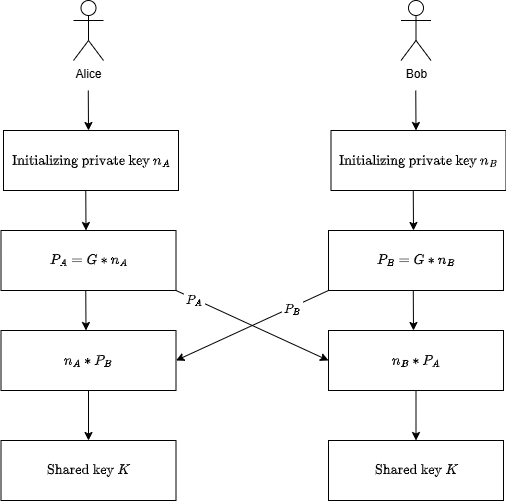
\includegraphics[width=0.8\textwidth]{flowcharts/eccdh.png} 
	\caption{Lược đồ Trao đổi khóa sử dụng giao thức khóa thỏa thuận ECCDH} 
	\label{fig:secp256k1}
\end{figure}

\subsubsection{Mã hóa/Giải mã}

\begin{figure}[H]
	\centering
	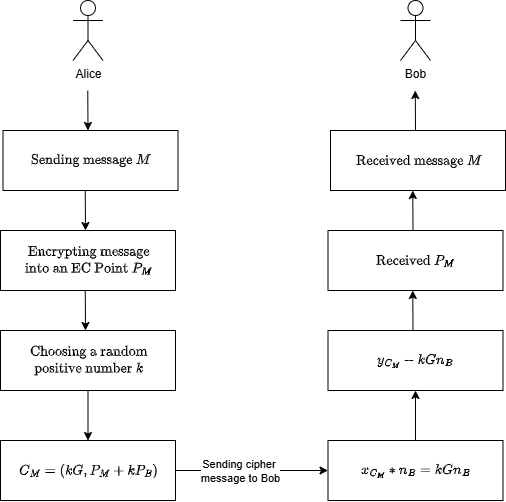
\includegraphics[width=0.8\textwidth]{flowcharts/ecc_elgamal.png} 
	\caption{Lược đồ Mã hóa/Giải mã bất đối xứng sử dụng Hệ mật mã trên đường cong Elliptic} 
	\label{fig:ecc_elgamal}
\end{figure}

\section{Thuật toán hàm băm (SHA-256)}

SHA-2 là một họ hàm băm mật mã được Cơ quan An Ninh Quốc gia Hoa Kỳ (NSA) phát triển và được Viện Tiêu chuẩn và Công nghệ Quốc gia Hoa Kỳ (NIST) xuất bản trong Tiêu chí Xử lý Thông tin Liên bang (FIPS PUB 180-2) vào tháng 08-2002. \nocite{fips1802}

SHA-256 là một thuật toán mật mã thuộc họ SHA-2. SHA-256 được xây dựng dựa trên hàm băm Merkle–Damgård, là hàm mật mã chống va chạm được xây dựng từ các hàm nén một chiều chống va chạm. 

\subsection{Nguyên lý hoạt động}

Thuật toán SHA-256 là một hàm băm một chiều với cấu trúc lặp, được thiết kế để biến đổi đầu vào có kích thước bất kỳ thành một bản tóm tắt dữ liệu (message digest) duy nhất. 

Ưu điểm cốt lõi của thuật toán này là khả năng đảm bảo tính toàn vẹn của tin nhắn, trong đó mọi thay đổi dù nhỏ nhất cũng sẽ dẫn đến một bản tóm tắt hoàn toàn khác biệt. Vì thế, SHA-256 đóng vai trò quan trọng trong việc tạo chữ ký số, xác thực thông điệp và sinh số ngẫu nhiên (bits).

Quy trình băm của SHA-256 được mô tả qua hai công đoạn chính:
\begin{itemize}
	\item \textbf{Tiền xử lý (Preprocessing)}: Thực hiện đệm thông điệp (padding messages), phân tách dữ liệu đã được đệm thành các khối có kích thước cố định và thiết lập các giá trị khởi tạo ban đầu nhằm phục vụ cho tính toán băm.
	\item \textbf{Tính toán băm (Hash computation}): Tạo lịch trình tin nhắn (message schedule), kết hợp cùng các hàm logic, hằng số và phép toán trên từ mã để sinh ra các giá trị băm qua từng vòng lặp. Giá trị băm cuối cùng thu được cũng chính là đầu ra của hàm băm SHA-256.
\end{itemize}

Các kích thước của khối dữ liệu cũng như các từ được sử dụng trong quá trình băm được trình bày dưới bảng sau:

\begin{table}[H]
	\centering
	\caption{Các yêu cầu thông số của thuật toán SHA-256}
	\label{tab:sha256-specs-full}
	\begin{tabular}{|p{2cm}|p{2cm}|p{2cm}|p{1.5cm}|p{2cm}|p{1.5cm}|p{2cm}|}
		\hline
		\textbf{Thuật toán} & \textbf{Độ dài kết quả của dữ liệu (bits)} & \textbf{Độ dài trạng thái bên trong (bits)} & \textbf{Độ dài khối (bits)} & \textbf{Độ dài dữ liệu (bits)} & \textbf{Độ dài từ (bits)} & \textbf{Số lần lặp trong chu kỳ (bits)} \\ \hline
		SHA-256 & 256 & 256 & 512 & $< 2^{64}$ & 32 & 64 \\ \hline
	\end{tabular}
\end{table}

\subsubsection{Các hàm logic}

Các phép Toán học được áp dụng trong các hàm logic:
\begin{table}[H]
	\centering
	\caption{Các phép toán trong SHA-256}
	\label{tab:sha256-ops}
	\begin{tabular}{|l|l|l|}
		\hline
		\textbf{Ký hiệu} & \textbf{Phép toán} & \textbf{Mô tả chi tiết} \\ \hline
		$ROTR^n(x)$ & Xoay phải & Dịch chuyển vòng tròn $x$ sang phải $n$ bit. \\ \hline
		$SHR^n(x)$ & Dịch phải & Dịch $x$ sang phải $n$ bit, lấp đầy bên trái bằng bit 0. \\ \hline
		$x \oplus y$ & XOR & Phép toán Exclusive-OR theo từng bit. \\ \hline
		$x \wedge y$ & AND & Phép toán logic AND theo từng bit. \\ \hline
		$\neg x$ & NOT & Phép lấy bù (đảo bit) của $x$. \\ \hline
		$x = (a+b) \mod 2^{32} $ & Cộng Modulo & Phép cộng số nguyên không dấu modulo $2^{32}$. \\ \hline
	\end{tabular}
\end{table}	

SHA-256 sử dụng sáu hàm logic, các hàm đều xử lý với các từ 32~bit, được biểu diễn qua $x, y$ và $z$. Đầu ra của mỗi hàm sẽ là một từ 32~bit mới.

\begin{align}
	Ch(x,y,z) &= (x\land y)\oplus(\neg x \land z) \\
	Maj(x,y,z)&= (x\land y)\oplus(x\land z)\oplus(y\land z)\\
	\Sigma_0^{\{256\}} &= ROTR^{28}(x) \oplus ROTR^{13}(x) \oplus ROTR^{22}(x)\\
 	\Sigma_1^{\{256\}} &= ROTR^{6}(x) \oplus ROTR^{11}(x) \oplus ROTR^{25}(x)\\
	\sigma_0^{\{256\}} &= ROTR^{7}(x) \oplus ROTR^{18}(x) \oplus SHR^{3}(x)\\
	\sigma_1^{\{256\}} &= ROTR^{17}(x) \oplus ROTR^{19}(x) \oplus SHR^{10}(x)
\end{align}

\subsubsection{Hằng số}

Hàm băm SHA-256 sử dụng một chuỗi 64 từ (32~bit mỗi từ) làm hằng số, được biểu diễn dưới dạng $K_0^{\{256\}}, K_1^{\{256\}},..., K_{63}^{\{256\}}$. 

Mỗi từ được biểu diễn là 32~bit đầu tiên của phần thập phân của căn bậc ba 64 số nguyên tố đầu tiên, các giá trị cụ thể được liệt kê ở bảng \ref{tab:sha256-k-constants}.

\subsubsection{Tiền xử lý}

\paragraph{a. Đệm tin nhắn}\quad

Một tin nhắn $M$ (Đầu vào của thuật toán) cần phải được đệm trước khi qua công đoạn tính toán băm. Đệm tin nhắn giúp đảm bảo độ dài tin nhắn sau khi được đệm sẽ là một bội số của 512. 

Giả sử độ dài của một tin nhắn $M$ là $\ell$ bit. Thêm bit $1$ vào cuối tin nhắn, theo sau đó là $k$ bit 0, với $k$ là nghiệm nhỏ nhất không âm của phương trình $\ell+1+k\equiv 448\mod512$. Sau đó, thêm vào một khối 64~bit biểu diễn số $\ell$ dưới dạng nhị phân, khi này đã trở thành một đoạn tin nhắn được đệm với độ dài 512~bit.

\textbf{Ví dụ:} một tin nhắn $8~bit~ASCII$ với nội dung "\textbf{\textit{gtvt}}" có độ dài là $8*4 = 32~bit$, vì thế tin nhắn sẽ được đệm vào 1~bit, sau đó $448-(32+1) = 415$ bit 0, và cuối cùng là 64~bit biểu diễn độ dài của tin nhắn dưới dạng nhị phân (32~bit).

\[
\underbrace{01100111}_{\text{\textbf{"g"}}} \quad
\underbrace{01110100}_{\text{\textbf{"t"}}} \quad
\underbrace{01110110}_{\text{\textbf{"v"}}} \quad
\underbrace{01110100}_{\text{\textbf{"t"}}} \quad
1 \quad
\overbrace{00...00}^{415} \quad
\overbrace{00...0100000}^{64}_{\ell=32}
\]

\paragraph{b. Phân tích, xử lý tin nhắn đệm} \quad

Sau khi tin nhắn đã được đệm, tin nhắn đệm này cần phải được phân tách ra thành $N$ khối $m~bit$ trước khi thực hiện tính toán hàm băm.

Với thuật toán SHA-256, tin nhắn được đệm sẽ được phân tách ra thành $N$ khối $512~bit$ ($M^{(1)}, M^{(2)},...,M^{(N)}$). Với mỗi khối đầu vào 512~bit, chúng sẽ được biểu diễn qua 16 từ 32~bit, 32~bit đầu tiên của khối tin nhắn $i$ được kí hiệu là $M_0^i$, 32~bit tiếp theo được kí hiệu là $M_1^i$, và cứ tiếp tục cho đến  $M_{15}^i$.

\paragraph{c. Thiết lập giá trị băm khởi tạo}\quad

Trước khi tính toán băm, cần phải thiết lập giá trị băm khởi tạo $H^{(0)}$.

Giá trị băm khởi tạo $H^{(0)}$ trong thuật toán SHA-256, bao gồm 8 từ 64~bit 	được biểu diễn dưới dạng thập lục phân.

Tám từ này tương ứng với 64~bit đầu tiên của phần thập phân của căn bậc hai tám số nguyên tố đầu tiên. 

\begin{align*}
	H_0^{(0)} &= 6a09e667 \\
	H_1^{(0)} &= bb67ae85 \\
	H_2^{(0)} &= 3c6ef372 \\
	H_3^{(0)} &= a54ff53a \\
	H_4^{(0)} &= 510e527f \\
	H_5^{(0)} &= 9b05688c \\
	H_6^{(0)} &= 1f83d9ab \\
	H_7^{(0)} &= 5be0cd19 \\	
\end{align*}
\subsubsection{Tính toán băm}

Sau quá trình tiền xử lý, với mỗi khối tin nhắn $M^{(1)}, M^{(2)},...,M^{(N)}$, sẽ được xử lý theo tuần tự qua các bước sau:

\begin{enumerate}[label=\textbf{Bước \arabic*:}, leftmargin = 2.5cm]
	\item Mở rộng lịch trình tin nhắn $\{W_t\}$:
		\[
		W_t = \begin{cases} 
				M_t^{(i)} & 0 \leq t \leq 15 \\
				\sigma_1^{\{256\}}(W_{t-2}) + W_{t-7} + \sigma_0^{\{256\}}(W_{t-15}) + W_{t-16} & 16 \leq t \leq 63 
			  \end{cases}
		\]
	Với $M_t^{(i)}$ là từ được lấy từ khối tin nhắn 512~bit và $W_t$ là từ 32~bit được tạo từ công thức trên.
	
	\item Khởi tạo 8 biến làm việc $a,b,c,d,e,f,g,h$, với vị trí nơi các từ sẽ được lưu trữ trong quá trình nén.
	
	\begin{align*}
a &= H_0^{(i-1)} \quad & e &= H_4^{(i-1)} \\
b &= H_1^{(i-1)} \quad & f &= H_5^{(i-1)} \\
c &= H_2^{(i-1)} \quad & g &= H_6^{(i-1)} \\
d &= H_3^{(i-1)} \quad & h &= H_7^{(i-1)}
	\end{align*}

	\item Tiến hành chạy chu kỳ nén qua các quá trình tính toán sau, thực hiện chu kỳ này từ $t = 0~ \text{đến} ~t = 63$:
	
	\begin{align*}
		T_1 &= h + \Sigma_1^{\{256\}}(e)+Ch(e,f,g)+K_t^{\{256\}}+ W_t \\
		T_2 &= \Sigma_0^{\{256\}}(a) + Maj(a,b,c) \\
 	
	\end{align*}
	Trong đó:
		\begin{itemize}
			\item $T_1~ \text{và} ~T_2$: Hai biến tạm được sử dụng để tính toán theo từng chu kỳ.
			\item $a,b,c,d,e,f,g,h$: Các biến làm việc.
			\item $K_t^{\{256\}}$: Hằng số theo chu kỳ $t$.
			\item $W_t$: Từ trong lịch trình tin nhắn.
		\end{itemize}
	\item Tính toán giá trị băm trung gian $H^{(i)}$ thứ $i$:
		\begin{align*}
		H_0^{(i)} &= a + H_0^{(i-1)} \quad & H_4^{(i)} &= e + H_4^{(i-1)} \\
	H_1^{(i)} &= b + H_1^{(i-1)} \quad & H_5^{i} &= f + H_5^{(i-1)} \\
		H_2^{(i)} &= c + H_2^{(i-1)} \quad & H_6^{(i)} &= g + H_6^{(i-1)} \\
		H_3^{(i)} &= d + H_3^{(i-1)} \quad & H_7^{(i)} &= h + H_7^{(i-1)}
	\end{align*}
	\item Lặp lại từ bước 1 đến bước 4 $N$ lần, sau đó chuyển đổi các giá trị băm dưới dạng hệ thập lục phân và nối các giá trị này lại với nhau, và chúng cũng chính là đầu ra của thuật toán băm SHA-256:
		\begin{center}
			$H_0^{(N)} \parallel H_1^{(N)} \parallel H_2^{(N)} \parallel H_3^{(N)} \parallel H_4^{(N)} \parallel H_5^{(N)} \parallel H_6^{(N)} \parallel H_7^{(N)}$
		\end{center}
\end{enumerate}

\subsection{Mã giả}

\subsubsection{Tiền xử lý}

	MessagePreprocessing(M):\\
	
			padded\_message = PaddingMessage(M): Đệm tin nhắn $M$ ban đầu sao cho tổng độ dài sau khi đệm là có tổng độ dài là một bội số của 512~bit.\\
		
			ParsingPaddedMessage(padded\_message): Chia M đã được đệm thành N khối 512 bit, mỗi khối là 16 từ 32 bit.\\
			
			HashValueInitialization(): Khởi tạo giá trị băm $H^{(0)}$.

\subsubsection{Tính toán băm}

	HashComputation:\\
	
		for i=1 to N:\\
		
		\{
		
		\qquad \textbf{Tạo lịch trình tin nhắn, $\{W_t\}$:}
			\[
			W_t = \begin{cases} 
				M_t^{(i)} & 0 \leq t \leq 15 \\
				\sigma_1^{\{256\}}(W_{t-2}) + W_{t-7} + \sigma_0^{\{256\}}(W_{t-15}) + W_{t-16} & 16 \leq t \leq 63 
			\end{cases}
			\]
		
		\qquad \textbf{Khởi tạo các biến làm việc:}
			\begin{align*}
				a &= H_0^{(i-1)} \quad & e &= H_4^{(i-1)} \\
				b &= H_1^{(i-1)} \quad & f &= H_5^{(i-1)} \\
				c &= H_2^{(i-1)} \quad & g &= H_6^{(i-1)} \\
				d &= H_3^{(i-1)} \quad & h &= H_7^{(i-1)}
			\end{align*}
			
		\qquad \textbf{Thực hiện chu kỳ nén:}\\
		
			\qquad \qquad for t=0 to 63:
			
			\qquad \qquad \{
			
				\begin{align*}
					T_1 &= h + \Sigma_1^{\{256\}}(e)+Ch(e,f,g)+K_t^{\{256\}}+ W_t \\
					T_2 &= \Sigma_0^{\{256\}}(a) + Maj(a,b,c) \\
					h &= g \\
					g &= f \\
					f &= e \\
					e &= d + T_1 \\
					d &= c\\
					c &= b\\
					b &= a\\
					a &= T_1 + T_2
				\end{align*}
				
			\qquad \qquad \}
			
		\qquad \textbf{Tính giá trị băm trung gian $H^{(i)}$:}
		
		\begin{align*}
			H_0^{(i)} &= a + H_0^{(i-1)} \quad & H_4^{(i)} &= e + H_4^{(i-1)} \\
			H_1^{(i)} &= b + H_1^{(i-1)} \quad & H_5^{i} &= f + H_5^{(i-1)} \\
			H_2^{(i)} &= c + H_2^{(i-1)} \quad & H_6^{(i)} &= g + H_6^{(i-1)} \\
			H_3^{(i)} &= d + H_3^{(i-1)} \quad & H_7^{(i)} &= h + H_7^{(i-1)}
		\end{align*}
		
	\}\\
	
	\textbf{SHA-256 Output} = $H_0^{(N)} \parallel H_1^{(N)} \parallel H_2^{(N)} \parallel H_3^{(N)} \parallel H_4^{(N)} \parallel H_5^{(N)} \parallel H_6^{(N)} \parallel H_7^{(N)}$

\subsection{Flowchart}

\subsubsection{Luồng hoạt động tổng quan}

\begin{figure}[H]
	\centering
	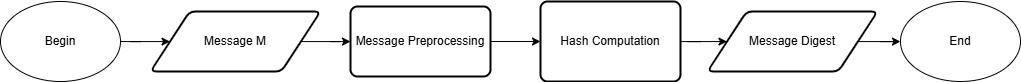
\includegraphics[width=\textwidth]{flowcharts/SHA-256-OVR.png} 
	\caption{Quy trình thuật toán băm SHA-256 hoạt động} 
	\label{fig:sha256_ovr}
\end{figure}

\subsubsection{Cấu trúc tin nhắn đệm}

\begin{figure}[H]
	\centering
	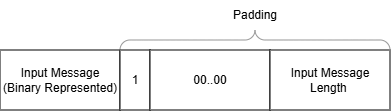
\includegraphics[width=0.8\textwidth]{flowcharts/Padding_Message.png} 
	\caption{Tin nhắn đầu vào đã được đệm} 
	\label{fig:padding_message}
\end{figure}

\subsubsection{Tạo lịch trình tin nhắn}

\begin{figure}[H]
	\centering
	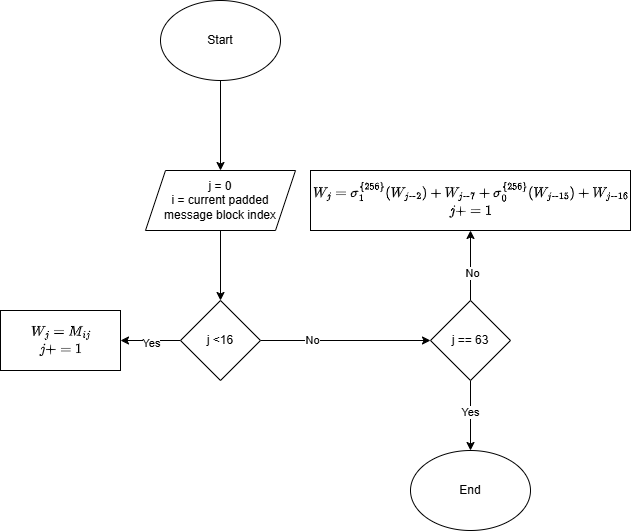
\includegraphics[width=\textwidth]{flowcharts/message_schedule.png} 
	\caption{Quy trình tạo lịch trình tin nhắn} 
	\label{fig:message_schedule}
\end{figure}

\subsubsection{Chu kỳ nén}

\begin{figure}[H]
	\centering
	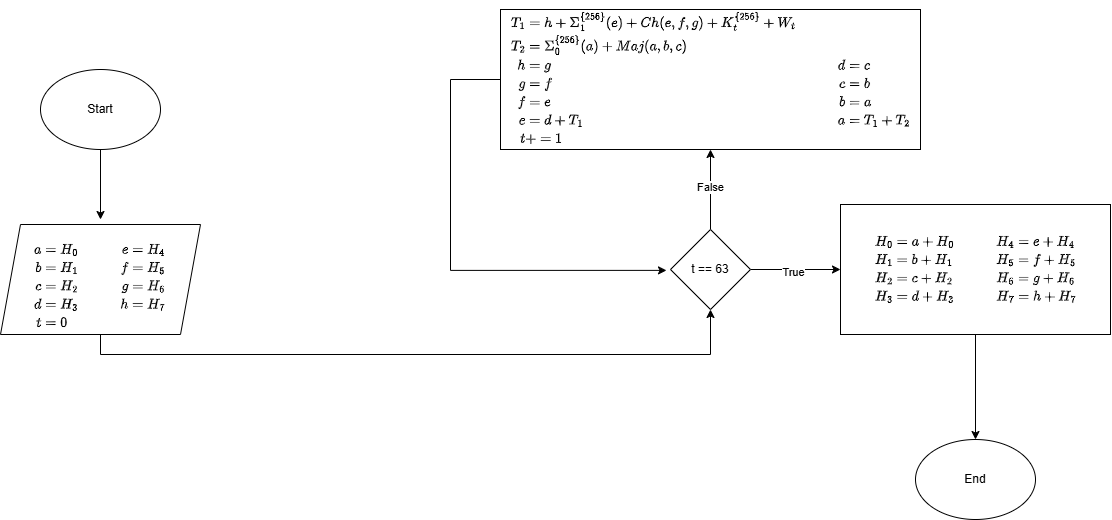
\includegraphics[width=\textwidth]{flowcharts/compression_hash.png} 
	\caption{Chu kỳ nén trong tính toán hàm băm} 
	\label{fig:compression_hash}
\end{figure}

\subsubsection{Tính toán hàm băm}

\begin{figure}[H]
	\centering
	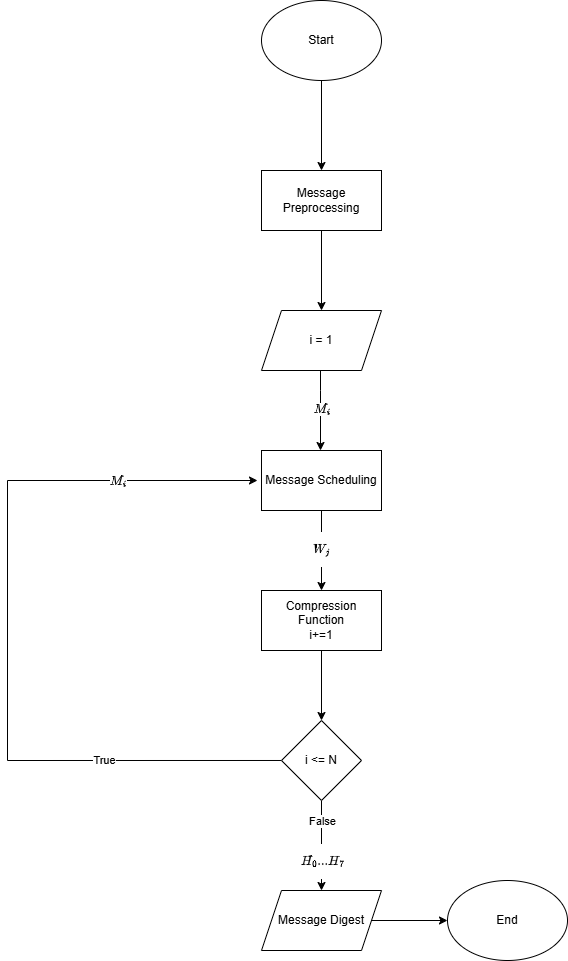
\includegraphics[width=0.8\textwidth]{flowcharts/hash_computation.png} 
	\caption{Tổng quan quá trình tính toán hàm băm} 
	\label{fig:hash_computation}
\end{figure}


\section{Thuật toán chữ ký số}

Lược đồ chữ ký số Schnorr là một hệ thống chữ ký số nổi tiếng và là hệ thống đầu tiên có tính bảo mật thông qua phát hiện các bài toán logarithm rời rạc cụ thể.

Nhờ vào khả năng giảm thiểu khả năng tính toán phụ thuộc vào kích thước thông điệp để tạo ra chữ ký, lược đồ chữ ký số Schnorr có thể tạo ra các chữ ký ngắn gọn nhưng đạt hiệu quả.

\subsection{Thủ tục sinh khóa}

Các bước của thủ tục này nhằm tạo ra cặp khóa riêng tư - khóa công khai:
\begin{enumerate}[label=\textbf{Bước \arabic*:}, leftmargin = 2.5cm]
	\item Chọn một số nguyên tố $p$ và $q$, sao cho $q$ là thừa số nguyên tố của $p-1$.
	\item Chọn một số $\alpha$, sao cho $\alpha^q = 1 \mod p$. Các tham số $\alpha, p, q$ và bộ khóa toàn cầu có thể được dùng chung với một nhóm người dùng.
	\item Chọn một số nguyên dương $s<q$, đây là khóa riêng của người gửi.
	\item Khóa công khai của người gửi: $v = \alpha^{-s} \mod p$
\end{enumerate}

\subsection{Quy trình ký}

Sau khi người gửi có khóa riêng - khóa công khai, tương ứng với $s ~\text{và}~ v$, quy trình tạo chữ ký như sau:

\begin{enumerate}[label=\textbf{Bước \arabic*:}, leftmargin = 2.5cm]
	\item Chọn một số nguyên $r$ ngẫu nhiên sao cho $0<r<q$ và tính $x = \alpha^{-r} \mod p $.
	\item Đính kèm thông điệp $M$ cần ký với $x$ và băm chúng để tính giá trị $e$: $e = H(M||x)$. ($H$ chính là hàm băm).
	\item Tính $y = (r+se) \mod q$.
	\item Chữ ký sau khi được tạo chính là cặp $(e,y)$

\end{enumerate}

\subsection{Quy trình xác nhận}

Để bên người nhận có thể xác nhận tin nhắn, thực hiện:

\begin{enumerate}[label=\textbf{Bước \arabic*:}, leftmargin = 2.5cm]
	\item Tính $x' = \alpha^{y}v^e\mod p$.
	\item Xác nhận $e = H(M||x')$
	\item $H(M||x') = H(M||x)$, tin nhắn kèm theo chữ ký của người gửi đã được bên người nhận xác nhận thành công.
\end{enumerate}

Cách $H(M||x') = H(M||x)$ được thể hiện thông qua phương trình sau đây:

\begin{center}
	$x' \equiv \alpha^{y}v^e \equiv \alpha^{y} \alpha^{-se} \equiv \alpha^{y-se} \equiv \alpha^r \equiv x(\mod p)$
\end{center}

\subsection{Flowchart}

\subsubsection{Thủ tục sinh khóa}

\begin{figure}[H]
	\centering
	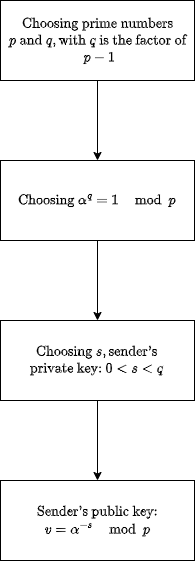
\includegraphics[width=0.4\textwidth]{flowcharts/schnorr_keygen.png} 
	\caption{Thủ tục sinh khóa lược đồ chữ ký số Schnorr} 
	\label{fig:schnorr_keygen}
\end{figure}


\subsubsection{Quy trình ký / quy trình xác nhận}

\begin{figure}[H]
	\centering
	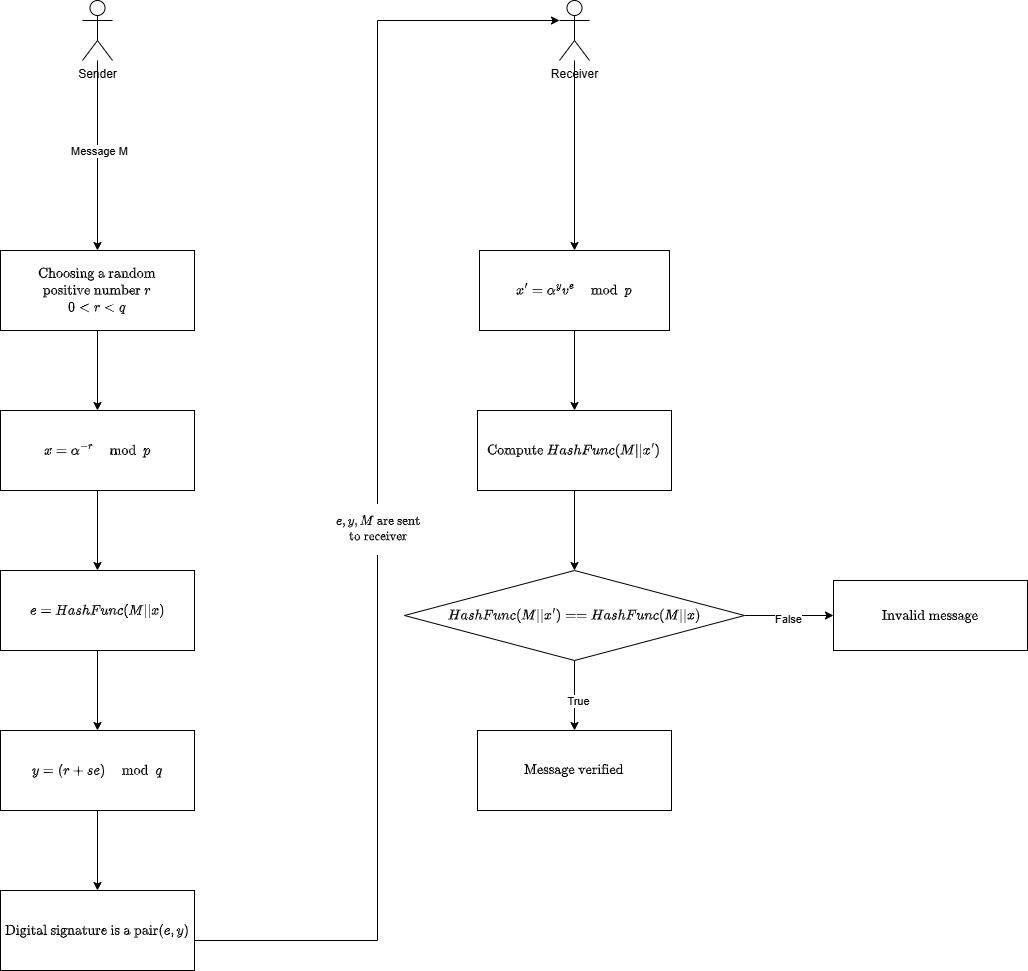
\includegraphics[width=0.9\textwidth]{flowcharts/schnorr_ds_scheme.png} 
	\caption{Lược đồ quy trình ký và xác nhận trong lược đồ Schnorr} 
	\label{fig:schnorr_sign_verify}
\end{figure}

